
%% the meat of your thesis is generally composed in these next three chapters
%% (overview, detailed work, analysis).  the breakdown is common across many
%% theses.

%% the (overview) chapter should give a high level overview of your thesis
%% topic.  there should have figures/illustrations and a high level discussion
%% of the key ideas of your work.  technically it should expand the discussion
%% of your work that you opened in the introduction.

%% the next chapter (detailed work) should explain all the nitty gritty details
%% of each part of your work.  the intro should describe each part that should
%% be followed by sections detailing each part.

%% finally the (analysis) chapter should detail the performance analysis and
%% performance results that you have performed.

%% now back to this overview chapter.

%% start with an introductory paragraph, what does this chapter cover?  if you
%% did not provide a plan of study in the intro chapter, then you will proabably
%% want to outline your research plan here.

\chapter{Implementation}\label{secrphash}

In this section we will describe the two main variants of the \textsf{RPHash} algorithm.  First we discuss the original
\textsf{2-Pass RPHash} algorithm designed for distributed processing on platforms such as Hadoop MapReduce.  Next we
discuss the \textsf{streamingRPHash} variant for streaming data designed for platforms such as Spark.

\section{Implementation Overview}

\textsf{RPHash} is a distributed algorithm for dense region and micro-cluster identification suitable as a precursor to
more robust clustering algorithms ($k$-Means, LDA, Mean Shift) or as a standalone approximate clustering algorithm.  In
the (\textsf{RPHash}) algorithm, both approximate and randomized techniques are employed to provide a stochastic element
to our clustering algorithm.  To combat the curse of dimensionality (COD), \textsf{RPHash} performs multi-probe, random
projection with Gaussian blurring of high dimensional vectors to the unique partitions of the Leech Lattice
($\Lambda_{24}$) \cite{Andoni}.

\subsection{Overview of the RPHash algorithm} 

The basic intuition of \textsf{RPHash} is to combine multi-probe random projection with discrete space quantization.
Following this intuition, near-neighbor vectors are often projected to the same partition of the space quantizer, which
is regarded as a hash collision in LSH parlance.  As an extension, multi-probe projection ensures that regions of high
density in the original vector space are projected probabilistically more often to the same partitions that correspond
to density modes in the original data.  In other words, partitions with high collision rates are good candidates for
cluster centroids.  To follow common parameterized $k$-means methods, the top $k$ densest regions will be selected.

According to the \emph{JL} lemma, the sub-projections will conserve the pairwise distances in the projected space for
points with $\epsilon$-distortion in which the size of the dataset is proportional to the logarithm of the number of
dimensions in the randomly projected subspace.  In addition to compressing a dataset to a computationally more feasible
subspace for performing space quantization, random projection can also make \emph{eccentric} cluster more spherical
\cite{Dasgupta2000,vempala}.

Discrete space quantizers play a central role in the \textsf{RPHash} algorithm.  The sequential implementation of the
\textsf{RPHash} algorithm will rely on the efficient Leech lattice decoder of Vardy, Sun, Be'ery, and Amrani
\cite{Vardy95,Sun,Be'ery,Amrani} used as a space quantizer.  The lattice decoder implementation relies on the
decomposition of the binary $(24,22,8)$ extended Golay Code into 4 partitions of the $(6,3,4)$ quaternary hexacode and
its relation to the Leech Lattice as a type B lattice construction.  This decomposition and relation to the Golay Code
provides a real worse case decoding complexity well below the asymptotically exponential bound for trellis decoders as
the dimension $d$ increases \cite{Tarokh1}.  The Leech lattice is a unique lattice in 24 dimensions that is the
densest lattice packing of hyper-spheres in 24 dimensional space \cite{leech,SPLAG}.  While the Leech lattice has many
exceptional properties, of particular importance to \textsf{RPHash} is that it provides the densest regular lattice
packing possible in 24 dimensions.  It was shown to be nearly optimal among even theoretical non-regular packings
\cite{Cohn} and more recently proven to be the densest packing achievable in $\mathbb{R}^{24}$ \cite{cohn2016}.  The 24
dimensional subspace partitioned by the Leech Lattice is small enough to exhibit the spherical clustering benefit of
random projection.  Low distortion random embeddings are also feasible for very large dataset ($n = \Omega(c^{24})$) to
lower dimensions (shown in \cite{bartal}), however for projective clustering at much lower embeddings, these embeddings
risk exhibiting the the occultation problem of \cite{Urruty2007}.  Furthermore, the decoding of the Leech lattice is a
well studied subject with a constant worse case decoding complexity of 331 operations \cite{Vardy95}.

Space quantizers have hard margin boundaries and will only correctly decode points that are within the error correcting
radius of its partitions.  This is an an issue found in approximate nearest neighbor search \cite{panigrahy,Andoni} and
is overcome in a manner similar to Panigrahy \cite{panigrahy} --- by performing multiple random projections of a vector
and then applying the appropriate locality sensitive to provide a set of hash IDs.  Using multiple random projections of
a vector allows the high dimensional vector to be represented as `fuzzy' regions that are probabilistically dependent on
the higher dimensional counterpart.  From Panigrahy \cite{panigrahy}, the requirement of ($\Theta(log(n))$) random
projection probes is given to achieve c-approximate hash collisions for the bounded radius, r-near vectors.  Random
projection probing adds a $\Theta(log(n))$-complexity coefficient to the clustering algorithm.  The top $k$ cardinality
set of lattice hash ID vector subsets represent regions of high density.

Projected clustering of representative cluster centroids will not in general be correlated with other projections of
data into projected cluster centroids.  To recover data from the projection step, we must map projected vectors back to
their original un-projected data space counterparts. The original data space vectors can then used to compute centroids
corresponding to the clusters in the projected space.  Figure \ref{lowtohigh} shows an example of this process for 3
projection probes of $\mathbb{R}^{3}\rightarrow \mathbb{R}^2 \rightarrow \mathbb{R}^3$.  Any off-line clustering
algorithm can be performed to resolve the overestimate of $k$ the number of desired clusters, effectively merging the
$k\times \text{number of projections}$ representations of centroids in the original data space.

An outline of the steps in the main steps of the \textsf{RPHash} algorithm (Algorithm \ref{2passrp}) is given below.  One
way that the \textsf{RPHash} algorithm achieves scalability is through the region assignment.  Clustering region
assignments are performed by decoding vector points into partitions of the Leech Lattice.

In most cases the problem space will not be exactly 24 dimensional.  The Johnson-Lindenstrauss (\emph{JL}) lemma and
subsequently, random projection provides a solution to this problem and provides additional benefits (See Section \ref{rpprelim}).
\emph{JL} states that for an arbitrary set of n points in m dimensional space, a projection exists onto a d-dimensional
subspace such that all points are linearly separable with $\epsilon$-distortion following $d \propto {\Omega({\frac{
      log(n) } {\epsilon^2 log 1/\epsilon} })}$.  Although many options for projections exists, a simple and sufficient
method for high dimensions is to form the projection matrix $r_{ij}\in\textbf{R}$ is $m\times d$ as follows:
\[
    r_{ij}= 
\begin{cases}
    +1, & \text{with probability } {\frac{1}{6}}\\
     0, & \text{with probability } {\frac{2}{3}}\\
    -1, & \text{with probability } {\frac{1}{6}}\\
\end{cases}\text{\ \ \ \ \cite{Achlioptas01}}
\]
Although the Leech lattices partitions provide optimal sphere packing in 24 dimensions for regular lattices, (an
unrelated version of the curse of dimensionality) the overall density of the lattice is sparse at $ 0.001930 $.  To
overcome this, \textsf{RPHash} ``blurs'' the projected data by apply shifts to projected vectors to more fully cover the
$\mathbb{R}^{24}$ subspace and performing multiple probes of the Leech Lattice partitions in addition to the vector
$v_{24}$ : $v_{24} = \{ v_{24}, v_{24}+N(0,1)_{24}... \}$ .  The approximation of a random projection is computationally efficient for large datasets, and unlike a truly Gaussian
projection matrix, yields a semi-positive definite projection matrix, that is useful in showing the convergence of
\textsf{RPHash}.

\subsection{Blurring}

\begin{figure*}
  \centerline{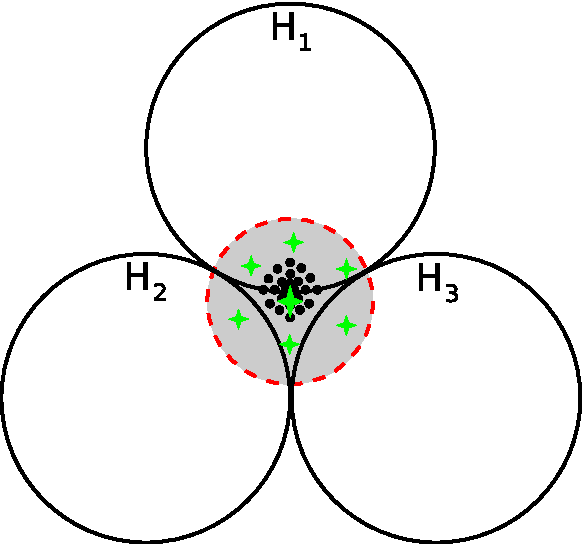
\includegraphics[width=.5\textwidth]{figs/blurring}}
  \caption{Gaussian Blurring to Fill Sparse Lattices.}\label{blurring}
\end{figure*}

Another way to overcome the hard-margins region assignments induced by a discrete lattice is to generate random points
in an $r/2$ radius around the projected vector.  This perturbation about the projected vector results in an approximate
probability density region around the data point.  In order to achieve an approximate radius probing in all dimensions,
we add a Gaussian vector having elements $\{n_1, n_2, ..., n_d\}\in R$, where $\|R\|\approx r$ and is composed of
elements $n \in N(0,r)$.

\subsection{Multi-Projection Re-Association}\label{occultationSection}

Re-association with the original vectors is used to recover the final centroids as shown in Figure \ref{lowtohigh}.
However, we must now resolve the common case where low dimensional representations of re-associated vectors are
unrelated to those of other projections.  A simple solution found in \cite{braverman} and in other streaming algorithms
is to merge the over-estimated centroid set in an off-line step such as weighted $k$-means.  The off-line step merges
the $k\times \text{number of projections}$ representations of candidate centroids but in the original dimensional
embedding.

\begin{figure}
    \centerline{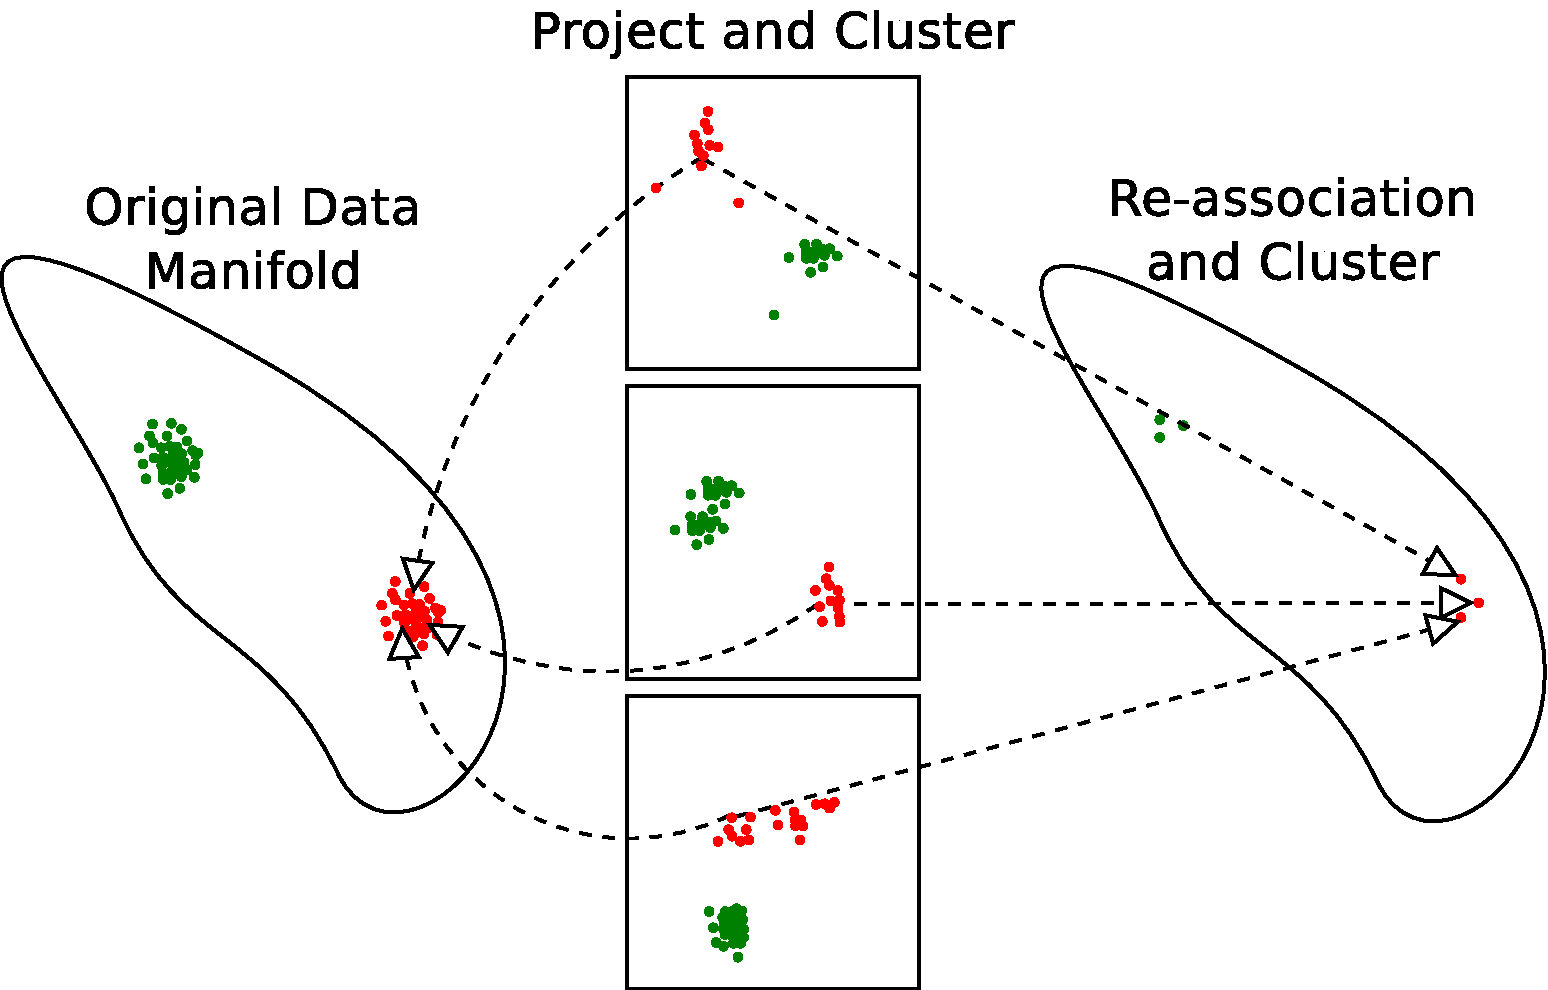
\includegraphics[width=.8\textwidth]{figs/LowToHigh}}
    \caption{Multiple projections $\mathbb{R}^{3}\rightarrow \mathbb{R}^2 \rightarrow \mathbb{R}^3$}\label{lowtohigh}
\end{figure}

A problem known as occultation arises when disjoint clusters in a $d$-dimensional space have non-disjoint projections on
lower-dimensional subspaces of $\mathbb{R}^d$.  Specifically, the probability of a $u$-occultation for the
$d$-dimensional space projected to 1-dimensional subspace is: $pr(u) = 1-{\frac{2}{\pi}} arcos({\frac{r_1+r_2}{d-c}})$,
where $r_1, r_2$ are radii of the respective clusters, and $d-c$ is the distance between them \cite{Urruty2007}.  The
method employed in \cite{Urruty2007} is to repeat the projection until a non-occulting projection is found.  The rate of
convergence for finding a non-occulting projection is given as:

$$\underset {d\rightarrow \infty}{lim}1-\bigg({\frac{2(r_1+r_2)} {\pi \|d-c\|}}\bigg)^d = 1$$ \label{occultation}

\noindent
which is exponential in $d$.  Recognized in \cite{Urruty2007}, this bound is slightly more favorable for an orthogonal
projection than the convergence rate of multiple single projections, as the distinct random projections are not always
linearly independent.  For certain decoders like the Leech Decoder and Spherical LSH, the required 24 and 32-dimensional 
projection is nearly orthogonal when the projection matrix is constructed of Gaussian random variables \cite{vempala}.


\RestyleAlgo{boxruled}
%%\begin{figure}[h]
%% \caption*{Data}
%%  $K$ - number of clusters\\
%%  $X=\{x_1,...,x_n\}$, $x_k \in \mathbb{R}^m$ - data vectors\\
%%  $ C$- a $k$-HH counter\\
%%  $\mathbb{H}$ - LSH Function\\
%%  $\mathbb{P} = \{p_1,...p_n\}$ - set of projection matrices\\
%%  $L=\{\{\varnothing\}...\}$\\
%%  $M = \{C,[0,...0]\}$\\
%%\end{figure}
%%\RestyleAlgo{boxruled}

\begin{algorithm}
\caption{ 2-Pass \textsf{RPHash} Algorithm\label{2passrp}}
\KwData{\ \\
  $K$ - number of clusters\\
  $X=\{x_1,...,x_n\}$, $x_k \in \mathbb{R}^m$ - data vectors\\
  $ C$- a $k$-HH counter\\
  $\mathbb{H}$ - LSH Function\\
  $\mathbb{P} = \{p_1,...p_n\}$ - set of projection matrices\\
  $L=\{\{\varnothing\}...\}$\\
  $M = \{C,[0,...0]\}$\\}

\ForAll{$x_k \in X$} 
{
  \ForAll{$p_i \in \mathbb{P}$} 
  {
    $\tilde{x_k}\leftarrow \sqrt{\frac{m}{d}}p_i^{\intercal}x_k $\\
    $t = \mathbb{H}(\tilde{x_k})$\\
    $L[k][i] = t$\\
    $C$.add($t$)\\
  }
}
\ForAll{$x_k \in X$}
{
  \ForAll{$c_i \in C$.top($K$)}
  {
    \If{$L[k] \cap M[i][0] \neq 0$}
    {
	$\Delta = M[k]-x_k$\\
	$M[k]=M[k]+\Delta/count$\\
	$L[k]$.add($M[i][0]$)\\
    }
  }
}
 \KwResult{$M$ }
\end{algorithm}

\begin{figure}
    \centerline{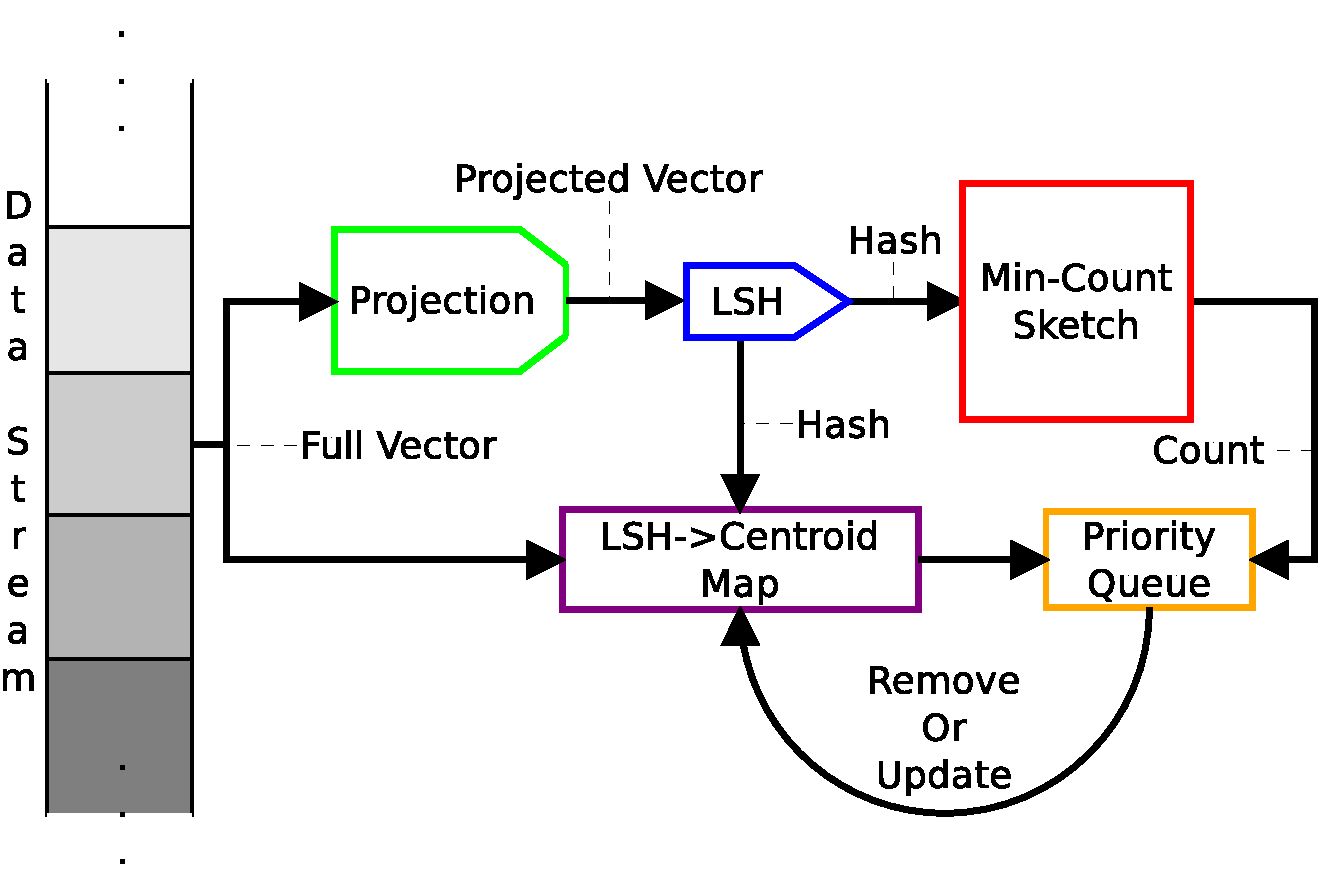
\includegraphics[width=.8\textwidth]{figs/rphashoverview}}
    \caption{Streaming \textsf{RPHash} Diagram}\label{rphash}
\end{figure}

In addition to Achlioptas efficient random projection method for databases, a further reduction in the number of
operation required for random subspace projection called the Fast Johnson-Lindenstrauss Transform (FJLT)
\cite{ailon2006,Dasgupta,ailon2013} is currently an active area of research.  FJLT, and similar nearly optimal
projection methods, utilize the local-global duality (Heisenberg Principle) of the Discrete Fourier Transform to
precondition the projection matrix resulting in a nearly optimal number of steps to compute an $\epsilon$-distortion
random projection \cite{ailon2006,Dasgupta,ailon2013}.  A sub-linear bound on the number of operations required for the
dominant projection operation may further improve \textsf{RPHash}'s overall runtime complexity.  However it only becomes
beneficial when the vector dimensionality $d$ is very large.  For many clustering problems, this level of dimensionality is 
uncommon.

%Centroids are computed as the means of the subsets of data vectors prior to
%projection, in each region.

%\subsection{Clustering on Streaming Data and Approximate $k$-Heavy Hitters}

%To perform RPHash on a streaming dataset, the itemset counter must be bounded and able to quickly
%respond to itemset support queries. Formally, the \textbf{$k$-Heavy Hitters}(\emph{$k$-HH}) problem
%is the problem of identifying the $k$ most frequent items in a dataset. It can trivially
%be solved using a histogram with $\theta(n)$ space.  In the case of streams, distributed
%and big data, the space requirements are potentially infinite making the histogram
%approach infeasible.  In \cite{alon1996} the related distinct counting problem for
%streams, is shown to require $\theta(n)$ in the worst case.  As with many cases involving
%unbounded memory requirements, approximate approaches have been proposed such as
%\cite{Karp,Morris,Manku}.  A thorough survey of approximate distinct item counting and
%algorithms can be found in \cite{Cormode} where counting algorithms are partitioned in to
%two categories: Count based and sketch based.
%\begin{figure}
%    \centerline{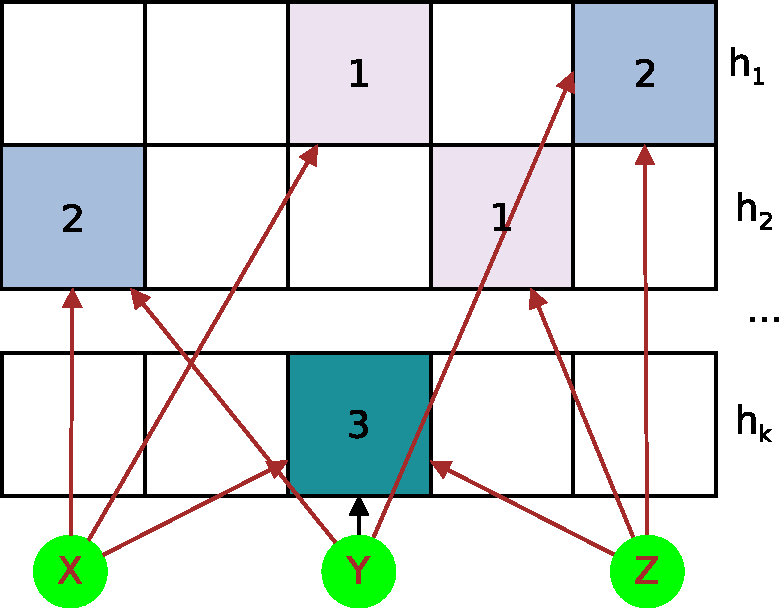
\includegraphics[width=.35\textwidth]{figs/countmin}}
%    \caption{Count-Min Sketch Algorithm}\label{countmin}
%\end{figure}
%One of the earliest streaming solutions for the approximate $k$-HH algorithms is the
%Count-min Sketch algorithm \cite{Cormode2}. Figure \ref{countmin} shows the primary data
%structure and action of the Count-min Sketch Algorithm for 3 elements $(X,Y,Z)$ and $k$
%hash functions.  Count-Min Sketch can be used to solve the approximate $k$-HH problem with
%only the additional of a priority queue using $\theta({1\over \epsilon} log {1 \over
%  \delta})$-space with error $(1-\epsilon)f$ where $f$ is the minimum frequency $m \over
%k$ to be consider frequent.

%Below we give the streaming version of the RPHash Algorithm. 

\subsection{Overview of \textsf{streamingRPHash}}

\textsf{streamingRPHash} is a stream clustering variant of the original 2-Phase \textsf{RPHash} algorithm of \cite{carraher-15}
which employs both approximate and randomized techniques to solve the $k$-means clustering problem.  To combat the curse
of dimensionality, \textsf{streamingRPHash} performs multi-probe, random projection with Gaussian blurring on high
dimensional data vectors \cite{Andoni}.

The general idea of \textsf{streamingRPHash} is motivated by a particular bad-case result in LSH based Nearest Neighbor
(LSH-NN) search where a single bucket contains an unprecedented number of candidate nearest neighbors.  This is a
problem in LSH-NN as the bucket then has to be linearly scanned for the optimal solution.  However, these degenerate
buckets can also be viewed as locally dense regions or density modes in the data.  Histograms offer a familiar 1-d
analog of our clustering solution.  A further advance of this considers not just the points within an arbitrary
histogram boundary, but relaxes the boundaries with a kernel based window function to smooth the overall population
density estimation.  A staple in kernel density estimation, the Parzen's window is a key motivation of the
\textsf{streamingRPHash} algorithm.

Due to the goal of providing an approximate solution to $\mathbb{R}^d$ for $d\gg1$, we must extend the windowing and
estimation techniques of Parzen's window to high dimensional space.  We could immediately apply the d-dimensional
hypercube partitioning and then count partition memberships.  But this method would suffer from many complexities
arising from the curse of dimensionality.  Similar to the issues encountered with k-d Tree NN \cite{marimont}, it will
also be computationally prohibitive and restricted by memory limitations.  \textsf{streamingRPHash} offers to mitigate
these issues by optimizing the approximate solution instead of the exact.

\textsf{streamingRPHash}, being motivated in part by LSH-NN, uses locality sensitive hash functions to partition the
data space evenly.  After both accuracy and time complexity tests, the 32-orthoplex spherical hash function was found to
be optimal across a wide range of datasets and system configurations.

An outline of the steps in the \textsf{streamingRPHash} algorithm are discussed below and summarized in Algorithm
\ref{streamingRPHashAlg}.  Some of the aspects of its function in regards to randomness and approximation are
highlighted here.  First, we discuss the generative nature of its region assignment.  Dense regions are identified by decoding data vectors
using a set of LSH functions.  In general the problem space will not match the locality sensitive hashing subspace.  The
previously described Johnson-Lindenstrauss (\emph{JL}) lemma offers a solution to this problem at the cost of a matrix
vector product.  Although \emph{JL}-lemma requires an $m\times d$ matrix of Gaussian random variables be formed,
\cite{Achlioptas01} suggests an approximate method to form the random projection matrix whose elements
$r_{ij}\in\textbf{R}$ have values from $\{1, 0, -1\}$ with probabilities $\{\frac{1}{6}, \frac{2}{3}, \frac{1}{6}\}$
respectively.  A further computational reduction is then achieved by treating the matrix-vector product as a linear scan
over the non-zero elements of the projection matrix, allowing us to effectively skip $\frac{2}{3}$ of the projection
computation, with the remaining $\frac{1}{3}$ operations consisting only of scalar additions.  Following this
computation, a scaling factor of ${\frac{1}{\sqrt{n}}}$ is also needed to preserve approximate distances between
projected vectors.

The subspace spanned by the 32-orthoplex is well below the requirements suggested by the \emph{JL}-bound for individual
vector discrepancy.  Fortunately, the effectiveness of projected $k$-means has been demonstrated successfully for
projections well below the \emph{JL}-bound (and well below $d = 32$) \cite{bartal,bingham}.  However, internal tests
show precision-recall performance drops as projection space dimensionality decreases.  To boost the overall data
retention of our clustering, we opt to perform multiple projections on original data vectors, followed by a
reconstruction step.  Similarly, a `blurring' step is used to increase the overall hash collision rate for nearby
vectors.  \textsf{streamingRPHash} `blurs' the projected data by applying shifts to projected vectors which help to
overcome the hard margins of the LSH decoder.

\section{\textsf{streamingRPHash} Algorithm} 

\textsf{streamingRPHash} follows the same structure as the original \textsf{RPHash} algorithm such as multiple random subspace
projections and their Re-Associations, Gaussian Blurring and LSH Functions.  However, the difference is in the way in
which \textsf{streamingRPHash} identifies and updates frequent density modes.  Due to the streaming data model's requirements
that an incoming data stream cannot be randomly accessed, or completely stored, we can only store a sketch of the
incoming data.  Furthermore, \textsf{streamingRPHash} cannot store the entire dataset, so the set of candidate centroids must be
bounded.  Fortunately, the Count-Min Sketch and its $k$-HH implementation fulfill both of these requirements.
The sequential version of the \textsf{streamingRPHash} algorithm is given in Algorithm \ref{streamingRPHashAlg}.

\begin{algorithm}
\RestyleAlgo{boxruled}
\KwData{\ \\
  $k$ - number of clusters\\
  $X=\{x_1,...,x_n\}$, $x_i \in \mathbb{R}^m$ - data vectors\\
  $M$- lsh\_key $\rightarrow$ centroid map \\
  $C$- cm-sketch data structure \\
  $T$- CM-Sketch based $\epsilon k$ bounded priority queue\\
    $R= \{r_1,...,r_{\log_2d}\}$, $r_i \in \mathbb{R}^d$ - Gaussian blurring vectors\\
  $\mathbb{H}(\cdot)$ - LSH Function\\
  $\mathbb{P} = \{p_1,...p_n\}$ - set of $n, m \times d $ projection matrices w/ \emph{JL} property\\}
\RestyleAlgo{boxruled}

\caption{\textsf{streamingRPHash} Algorithm\label{streamingRPHashAlg}}
\DontPrintSemicolon
\ForAll{$x \in X$} 
{
  \ForAll{$p \in \mathbb{P}$} 
  {
    $\tilde{x}:= \sqrt{\frac{m}{d}}p^{\intercal}x$ \tcp*{Random Projection}
    \ForAll{$r \in R$} 
      {
      $t := \mathbb{H}(\tilde{x}+r)$ \tcp*{LSH Hashing}
      $C$.add$(t)$\\
      \eIf{$t\in M$.keys}
      {
	$M[t].wadd(x)$  \tcp*{Weighted add}
      }
      {
	 $M[t]=$new centroid($x$,C.count(t))\\
	 $T$.insert$(M[t])$\\
      }
      M.remove(T.pop())  \tcp*{remove least}
    }
  }
}
\KwResult{OfflineWeightedClusterer($M$.items)}
\end{algorithm}

%% According to the \emph{JL} lemma, the sub-projections will conserve the pairwise
%% distances in the projected space for points with $\epsilon$-distortion in which the
%% size of the dataset is proportional to the logarithm of the number of dimensions in the
%% randomly projected subspace.  In addition to compressing a dataset to a computationally
%% more feasible subspace for performing space quantization, random projection can also
%% make \emph{eccentric} cluster more spherical \cite{Dasgupta2000,vempala}.

%The lattice decoder implementation relies on the decomposition of the binary $(24,22,8)$
%extended Golay Code into 4 partitions of the $(6,3,4)$ quaternary hexacode and its
%relation to the Leech Lattice as a type B lattice construction.  This decomposition and
%relation to the Golay Code provides a real worse case decoding complexity well below the
%asymptotically exponential bound for trellis decoders as the dimension $d$ increases
%\cite{Tarokh1,Tarokh2}.  The Leech lattice is a unique lattice in 24 dimensional space
%with many exceptional properties, however, of importance to \textsf{streamingRPHash} is
%that it is the densest regular lattice possible in 24 dimensions and nearly optimal among
%theoretical non-regular packings \cite{Cohn}.  The 24 dimensional subspace partitioned by
%the Leech Lattice is small enough to exhibit the spherical clustering benefit of random
%projection.  Low distortion random embeddings are also feasible for very large dataset
%($n = \Omega(c^{24})$) objects while avoiding the occultation phenomena
%\cite{Urruty2007}.  Furthermore, the decoding of the Leech lattice is a well studied
%subject, with a constant worse case decoding complexity of 331 operations \cite{Vardy95}.
%In addition to the Leech Lattice, other space quantizers exist with even better cr-NN
%performance for special types of spherically distributed data and the cosine distance.  A
%partitioning scheme of \cite{SLSH} uses the hypersphere surface partitioning of inscribed
%regular polytopes.  Although a variety of n-dimension regular polytope constructions
%exist, we choose the n-orthoplex for its simplicity, and relatively low number of
%partition regions ($2d$, compared to hypercube and simplex).  Furthermore, random
%rotations of the hypercube are used to generalize the partitioning, and on projected
%data, are already present in the projection matrix.

%Centroids are computed as the means of the subsets of data vectors prior to projection,
%in each region.  The approximation of a random projection matrix is not only
%computationally more efficient to generate, it also requires $frac{2}{3}$ fewer
%operations during the projection process., and unlike a projection matrix formed from
%truly Gaussian random variables, has an even better probability of yielding a positive
%semi-definite projection matrix at lower dimensions.

\section{$k$-HH}{Streaming Data and Approximate $k$-Heavy Hitters}

To apply \textsf{streamingRPHash} to data streams, the candidate centroid set must be bounded and able to quickly
respond to most frequent itemset queries.  Formally, the $k$-Heavy Hitters (\emph{$k$-HH}) problem is the problem of
identifying the $k$ most frequent items in a dataset \cite{cormode}.  It can trivially be solved using a histogram with
$\theta(n)$ space.  In the case of data streams, space requirements are potentially unbounded, making the histogram
approach infeasible.  In \cite{alon1996}, the related distinct counting problem for streams is shown to require
$\theta(n)$ space in the worst case.  As with many cases involving unbounded memory requirements, approximate approaches
have been proposed such as \cite{karp-03,morris-78,Manku}.  A thorough survey of approximate distinct item counting can
be found in \cite{cormode3} where counting algorithms are divided into two categories: \emph{count based} and
\emph{sketch based}.

One of the earliest streaming solutions for the approximate \emph{$k$-HH} algorithms is the Count-Min Sketch data
structure \cite{cormode2}.  Figure \ref{countmin} shows the primary data structure for 3 elements $(X,Y,Z)$ and $k$ hash
functions.  Count-Min sketch can be used to solve the approximate \emph{$k$-HH} problem with only the addition of a
priority queue using $\theta({1\over \epsilon} log {1 \over \delta})$ space with error $(1-\epsilon)f$, where $f$ is the
minimum frequency $m \over k$ to be considered frequent.

%\RestyleAlgo{boxruled}
%\begin{figure}[h]
% \caption*{Data}
%  $K$ - number of clusters\\
%  $X=\{x_1,...,x_n\}$, $x_k \in \mathbb{R}^m$ - data vectors\\
%  $ C$- a $k$-HH counter\\
%  $\mathbb{H}$ - LSH Function\\
%  $\mathbb{P} = \{p_1,...p_n\}$ - set of projection matrices\\
%  $L=\{\{\varnothing\}...\}$\\
%  $M = \{C,[0,...0]\}$\\
%  $r = \{r_0,...,r_{24}\}$ - random blur vector $\in \mathbb{R}^{24}$ \\
%\end{figure}
%\RestyleAlgo{boxruled}

%\begin{algorithm}
%\caption{Streaming Algorithm\label{streamingRPHashAlg}}
%\ForAll{$x_k \in X$} 
%{
%  \ForAll{$p_i \in \mathbb{P}$} 
%  {
%    \For{$b \in {{1}\over{D(\Lambda)}}$} 
%      {
%      $\tilde{x_k}\leftarrow \sqrt{\frac{m}{d}}p_i^{\intercal}x_k $\\
%      $t = \mathbb{H}(\tilde{x_k}+r)$\\
%      $tmp \rightarrow C$.top($K$).get($[t,x_k,0]$)\\
%      \eIf{tmp $\neq \varnothing$}
%      {
%	  $\Delta\leftarrow tmp[1]-x_k$\\
%	  $tmp[2]\leftarrow tmp[2]+1$\\
%	  $tmp[1]\leftarrow tmp[1] + \Delta/tmp[2]$\\
%      }
%      {
%	  $C$.add($[t,x_k,1]$)\\
%      }
%    }
%  }
%}
%\KwResult{$C$.top($K$)}
%\end{algorithm}

While the code base for \textsf{streamingRPHash} contains implementations for several LSH methods (including $E_8$,
Leech, and Spherical), our experimental studies show that the best overall performance is achieved with Spherical.
Hence the experiments in this dissertation report results with the spherical 32-orthoplex decoder of \cite{SLSH}.  The
spherical orthoplex decoding consists of a projection to 32$d$ space followed by a vector normalization step in order to
have the vector lie on the surface of a hypersphere.  Next, a random rotation is applied to the 64 basis vectors of the
32-orthoplex.  The basis vector nearest to the projected vector is then used as the vector's representative, and the
corresponding bits resulting from the natural ordering of basis vectors are used to define a $log_2(64)$ partial
decoding.  Subsequently, two similar additional hashings are applied to generate a total 18 bits of entropy.

%\RestyleAlgo{boxruled}
%\begin{algorithm}
%\caption{Streaming Algorithm\label{streamingRPHashAlg}}
%\ForAll{$x_k \in X$} 
%{
%  \ForAll{$p_i \in \mathbb{P}$} 
%  {
%    \For{$b \in {{1}\over{D(\Lambda)}}$} 
%      {
%      $\tilde{x_k}\leftarrow \sqrt{\frac{m}{d}}p_i^{\intercal}x_k $\\
%      $t = \mathbb{H}(\tilde{x_k})$\\
%      $tmp \rightarrow C$.top($K$).get($[t,x_k,0]$)\\
%      \eIf{tmp $\neq \varnothing$}
%      {
%	  $\Delta\leftarrow tmp[1]-x_k$\\
%	  $tmp[2]\leftarrow tmp[2]+1$\\
%	  $tmp[1]\leftarrow tmp[1] + \Delta/tmp[2]$\\
%      }
%      {
%	  $C$.add($[t,x_k,1]$)\\
%      }
%    }
%  }
%}
%\KwResult{$C$.top($K$)}
%\end{algorithm}

\section{Data Security}{Data Security: At no added cost}\label{security}

Recent United States government initiatives pushing for the large scale availability of data resources have made vast
quantities of de-identified health information available to the public.  These resources however have prompted advances
in attacks on de-identification of whole genome sequence data.  Such attacks have been used to associate, thought to be,
anonymous medical records with specific individuals \cite{deident}.  Similar de-anonymization attacks
\cite{deanon1,deanon2} along with a presidential commission (privacy and progress in WGS) have prompted a need for
better data security of medical records data.  The \textsf{RPHash} algorithm provides an intrinsic solution to this
problem in both the distribution of data among servers as well as during the communication steps required by the
algorithm.

While attempting to mitigate communication restrictions, \textsf{RPHash} intrinsically provides some security in the data
it exchanges.  Previous attempts at securing data in distributed systems required additional cryptographic steps
\cite{Lindell2000}.  Namely, the randomly projected centroid IDs, and the aggregation of only the $k$-largest cardinality
vector sets.  Non-distributed data clustering requires the entire dataset to reside on the processing system and
distributed methods often require communication of full data records between nodes.

In the subspace projection step of \textsf{RPHash}, nearly-orthogonal random projection is utilized as a destructive
operation, providing vector anonymity.  As a consequence of projecting the real data vectors to a random subspace via a
near, but not completely orthogonal matrix, destructive data loss occurs providing a cryptographic ``trapdoor''
function.  The data loss is an intrinsic part of the \textsf{RPHash} clustering algorithm that has little adverse effect
on its model generation and subsequent recall accuracy.  Given the likelihood that \textsf{RPHash} is applied to a dataset where
the number of vectors $n$ is much greater than the desired $k$ centroids, recovering an individual's private information
would require knowledge of $\frac{n}{k}$ (on average) records in the representative centroid.

\section{Software Implementation Details}

%% LEE: not really necessary and since it's just one paragraph, it's not a proper paragraph.  alternatively you could
%% expand it to multiple sentences and document the repos where everything lies.

%% RPHash and Variants of RPHash are provided in a variety of languages (Go, Python, and Java), however the primary
%% testing and performance analysis is performed on the Java variant.

%% LEE: is the abstaction from the abstract object \texttt{AbstractClusterer} or something else??  also, is it an
%% absract function or an abstract class??  please cleanup and check the names/capitalization of everything in the next
%% paragraph.  i tend to set references to code names in typewriter font.

\textsf{RPHash} and Variants of \textsf{RPHash} are provided in a variety of languages (Go, Python, and Java), however the primary
testing and development is done on the Java variant.  All software development and collaboration was
tracked using the git version control system and is made available on-line: 
\begin{itemize}
\item \url{https://github.com/wilseypa/rphash-java}
\item \url{https://github.com/wilseypa/rphash-spark}
\item \url{https://github.com/wilseypa/rphash-golang}
\item \url{https://github.com/leecarraher/PyRecRPHash}
\end{itemize}

The \textsf{RPHash} test frameworks is designed in \texttt{java} following an object-oriented approach.  Additional
performance metrics and algorithms for comparison are provided by various Matlab packages.
Common functional units with the similar functions are designed as implementations of general abstract classes (i.e 
\texttt{ArrayList} implements \texttt{List} functions)
Examples of abstract functional units that are described in more detail are \texttt{AbstractProjector},
\texttt{AbstractClusterer} , \texttt{AbstractDecoder}, and \texttt{AbstractCounter}.  The methods contained in each interface
pertain to their function within the \textsf{RPHash} \texttt{java} Framework.

The abstract class of all \textsf{RPHash} variants, which includes other clusterers for comparison is the \texttt{AbstractClusterer} class.
For algorithms specific to streaming datasets, a further abstraction of the \texttt{AbstactCluster} method is provided, \texttt{StreamingClusterer}
which amends the abstract clusterer with function prototypes for adding vectors in a stream and invoking the off-line process.  Implementing
clusterers in this framework allows us to easily design tests that are applicable to all \textsf{RPHash} variants and other clustering algorithms.

For implementation of the offline clustering and post processing clustering steps, multiple standard clustering
algorithms were implemented. These methods all implement the \texttt{AbstractClusterer} interface.  
In particular the following offline algorithms are included in the code base: Hartigan and
Wong $k$-Means \cite{Hartigan}, agglomerative clustering with single, complete average, and wards method link strategies,
Mean-Shift \cite{comaniciu-02}, Maximum Likelihood \cite{Hathaway}, DBScan \cite{dbscan}, $k$-Means++ \cite{arthur-07}, Braverman
\emph{et al} Streaming $k$-Means \cite{braverman} , Ailon \emph{et al} Streaming $k$-Means \cite{streamkmeans}, as well as a
dummy clusterer that simply samples the dataset.  All clustering methods can be wrapped in a multi-reseeding method that
optimizes within-cluster sum of squared error.

Multiple LSH algorithms were implemented for testing and comparison as implementations of the \texttt{AbstractDecoder} class. Decoders include 
the P-Stable-Distribution Decoder \cite{datar-04},
Spherical LSH Decoder \cite{SLSH}, Leech Decoder \cite{Andoni06,Amrani}, $E_8$ Decoder \cite{SPLAG}, the classic Dihedral Group Decoder\cite{SPLAG}, 
Origin Hamming Decoder \cite{indyk-98}, Binary Golay Decoder \cite{Amrani}, and or proposed Depth Probing Decoder.  All Decoders are composable into
multi-level decoders, through implementation of the multi-decoder wrapper.

\texttt{AbstractProjectors} consist of the DB-Friendly random projection method of \cite{Achlioptas01}, a the Gaussian variate based
projection \cite{vempala}, a bitwise DB-Friendly random projection method, the Fast
Johnson-Lindenstauss Transform \cite{ailon2006}, and the classic Principle Component projection.  

A set of counting and sketching
algorithms are also implemented in the \textsf{RPHash} test framework and are implementations of the \texttt{AbstractCounter} class.  
The included counting algorithms are: the Count-Min sketch \cite{cormode},
and its $k$-Heavy Hitter implementation \cite{cormode2}, Lossy counting \cite{morris-78} and a hash table based exact counter.  The
Count-Min implementation is adapted to also support vector sums and decay rates for streaming data in which clusters are regarded as
temporal structures.

For testing \textsf{RPHash}, a framework of statistical performance metrics and data generators and readers is provided.  The
generators consist mainly of Gaussian cluster generators, that can be sparse, heteroscedastic, and full or streaming.
All data readers implement a simple matrix format that supports both binary and ASCII data with uncompressed and LZ
compressed data.

